\begin{frame}[plain]
    \begin{bee}[Summary]
        \begin{enumerate}[1.]
            \item Introduction
                \begin{enumerate}[1.]
                    \item Context
                    \item Main Aims
                \end{enumerate}
            \item Concepts
                \begin{enumerate}[1.]
                    \item Ontologies
                    \item Resource Description Framework (RDF)
                    \item Web Ontology Language (OWL)
                    \item SPARQL Protocol and RDF Query Language (SPARQL)
                    \item Reasoning and Inference
                \end{enumerate}
            \item Challenges
            \item Schedule
        \end{enumerate}
    \end{bee} 
\end{frame}

\begin{frame}[plain]
    \begingroup
        \fontfamily{qag}\selectfont
        \Huge\color{black}\textbf{1. Introduction}\\[0.6em]
    \endgroup
\end{frame}

\begin{frame}{1.1 Context}
    \begin{bee}
        \begin{enumerate}[$\bullet$]
            \item In knowledge representation, \textbf{ontologies} provide a formal structure for concepts and relationships in a domain.
            \item Essential in AI, data integration, and the \textbf{Semantic Web} for consistent data linking.
            \item Growing data makes maintenance complex and ontologies can quickly become outdated or inconsistent.
            \item Expansion relies on \textbf{reasoners}, which can be computationally expensive, especially for large-scale or real-time updates.
    \end{enumerate}
    \end{bee}
\end{frame}

\begin{frame}{1.2 Main Aims}
    \begin{bee}
        \begin{enumerate}[$\bullet$]
        \item \textbf{Goal:} Develop an efficient engine for ontology expansion using \textbf{SPARQL CONSTRUCT} queries.
        \item \textbf{Phase 1:} Map ontological axioms to SPARQL queries for real-time inference and improved performance.
        \item \textbf{Phase 2:} Design a compiler to automatically generate those queries.
        \item \textbf{Outcome:}  
        \begin{enumerate}[$\bullet$]  
            \item Reduce manual effort in updates.  
            \item Reduce reliance on external reasoners.
            \item Improve speed and accuracy of knowledge integration.  
        \end{enumerate}
    \end{enumerate}
    \end{bee}
\end{frame}

\begin{frame}[plain]
    \begingroup
        \fontfamily{qag}\selectfont
        \Huge\color{black}\textbf{2. Concepts}\\[0.6em]
    \endgroup
\end{frame}

\begin{frame}{2.1 Ontologies}
    \begin{tikzpicture}[remember picture, overlay]
        \node at ([xshift=6cm,yshift=-4.5cm]current page.north west) {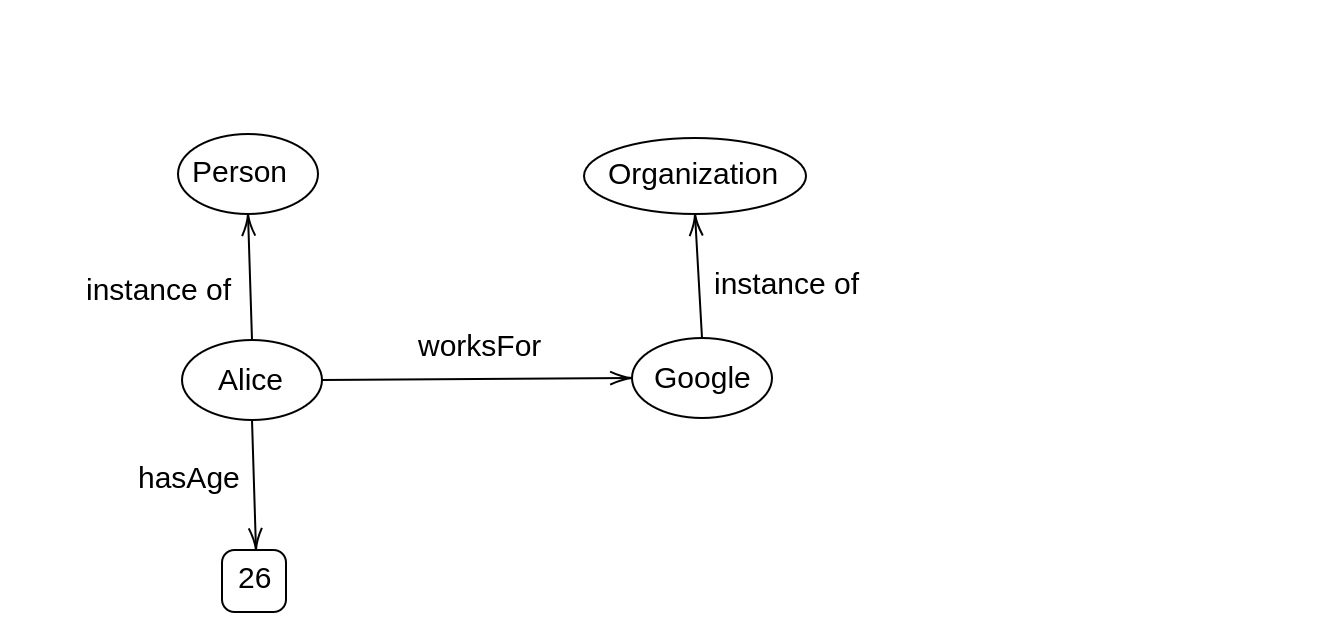
\includegraphics[width=12cm]{2-content/ontology-structure.png}};
    \end{tikzpicture}

    \begin{columns}
        \begin{column}{5cm}
        \end{column}
        \begin{column}{5cm}
            \begin{bee}[]
                Ontologies structure knowledge by defining concepts, relationships, and rules, enabling data standardization and human-machine understanding. They consist of classes, properties, and individuals.
            \end{bee}
        \end{column}
    \end{columns}
\end{frame}

\begin{frame}{2.2 Resource Description Framework (RDF)}
    \begin{bee}
        \begin{enumerate}[$\bullet$]
        \item \textbf{RDF:} Standard model for representing web data using triples \texttt{<subject, predicate, object>}.  
        \item \textbf{URIs:} Ensure unique identification of resources.  
        \item \textbf{RDFS:} Extends RDF with a vocabulary for structured data representation.  
        \item \textbf{Key RDFS Features:}  
        \begin{enumerate}[$\bullet$]
            \item \textbf{Classes and Instances:} Categorize resources.  
            \item \textbf{Properties:} Define relationships with domains and ranges.  
            \item \textbf{Hierarchy:} Support for subclass and subproperty relationships.  
        \end{enumerate}
    \end{enumerate}
    \end{bee}
\end{frame}

\begin{frame}{2.3 Web Ontology Language (OWL)}
    \begin{bee}
        \begin{enumerate}[$\bullet$] 
        \item Built on RDF to provide more expressiveness and support reasoning with ontologies.  
        \item Features of OWL:
        \begin{enumerate}[$\bullet$]
            \item \textbf{Class Hierarchies:} Supports subclass relationships, domain-specific taxonomies, and class constraints.  
            \item \textbf{Property Characteristics:} Define properties with transitivity, symmetry, functionality, and inverses.  
            \item \textbf{Axioms:} Allows logical reasoning through axioms to infer new knowledge.  
        \end{enumerate}
    \end{enumerate}
    \end{bee}    
\end{frame}

\begin{frame}{2.4 SPARQL Protocol and RDF Query Language (SPARQL)}
    \begin{bee}
        \begin{enumerate}[$\bullet$]
        \item Query language and protocol for RDF data to extract, filter, and construct data from RDF graphs.  
        \item SPARQL Components:
        \begin{enumerate}[$\bullet$]
            \item \textbf{SELECT:} Specifies the variables to retrieve. It is the core component for data extraction.  
            \item \textbf{CONSTRUCT:} Generates new triples based on query results, enabling data transformation.  
            \item \textbf{PREFIX:} Define namespaces to simplify URIs.  
            \item \textbf{WHERE:} Defines the triple pattern to match in the RDF graph.  
            \item \textbf{MODIFIERS:} Includes LIMIT, OFFSET, and ORDER BY to manipulate query results.  
        \end{enumerate}
    \end{enumerate}
    \end{bee}
\end{frame}

\begin{frame}{2.5 Reasoning and Inference}
    \begin{columns}
        \begin{column}{6cm}
            \begin{bee}[Reasoning]
                Computational application of inference, analyzing ontologies to deduce information or validate consistency. 
            \end{bee}
            \begin{bee}[Inference]
                Deriving new facts from existing knowledge using logical rules.  
            \end{bee}
        \end{column}

        \begin{column}{6cm}
            \begin{bee}[]
                Inference tasks include class inference, consistency checking, and property reasoning. However, limitations include incorrect inferences from inconsistent data and scalability issues with large datasets.
            \end{bee}
        \end{column}
    \end{columns}
\end{frame}

\begin{frame}[plain]
    \begingroup
        \fontfamily{qag}\selectfont
        \Huge\color{black}\textbf{3. Challenges}\\[0.6em]
    \endgroup
\end{frame}

\begin{frame}{3. Challenges}
    \begin{columns}
        \begin{column}{5cm}
            \begin{bee}[Efficiency]
                Reasoners may have slow performance with large or complex ontologies.
            \end{bee}
            
            \begin{bee}[SPARQL]
                Poor integration with SPARQL, limiting real-time decision-making. 
            \end{bee}
            
        \end{column}
        
        \begin{column}{5cm}
            \begin{bee}[Scalability]
                Struggle with large-scale ontologies, increasing resource demands. 
            \end{bee}
            
            \begin{bee}[Automation]
                Manual conversion of OWL axioms to SPARQL is error-prone, highlighting the need for automation.
            \end{bee}
        \end{column}
    \end{columns}
\end{frame}

\begin{frame}[plain]
    \begingroup
        \fontfamily{qag}\selectfont
        \Huge\color{black}\textbf{4. Schedule}\\[0.6em]
    \endgroup
\end{frame}

\begin{frame}{4. Schedule}

\begin{figure}[H]
    \centering
    \begin{ganttchart}[y unit title=0.35cm,
    y unit chart=0.4cm,
    vgrid,hgrid, 
    title label anchor/.style={below=-1.6ex},
    title left shift=.05,
    title right shift=-.05,
    title height=1,
    bar height=0.5,
    bar/.append style={draw=none, fill=black!65},
    group left shift=0,
    group right shift=0,
    group height=0.5,
    group peaks tip position=0,
]{1}{20}
    %labels
    \gantttitle{2024}{6} \gantttitle{2025}{14}\\
    \gantttitle{Out}{2}
    \gantttitle{Nov}{2}
    \gantttitle{Dec}{2}
    \gantttitle{Jan}{2}
    \gantttitle{Feb}{2}
    \gantttitle{Mar}{2}
    \gantttitle{Apr}{2}
    \gantttitle{May}{2}
    \gantttitle{Jun}{2}
    \gantttitle{Jul}{2} \\
    %tasks
    \ganttgroup{Preparation}{2}{6}\\
    \ganttbar{\textcolor{gray}{Requirements}}{2}{4} \\
    \ganttbar{\textcolor{gray}{Analysis}}{2}{6} \\
    \ganttbar{\textcolor{gray}{Technologies}}{3}{4} \\
    \ganttgroup{Development}{5}{14}\\
    \ganttbar{\textcolor{gray}{Architecture}}{5}{6} \\
    \ganttbar{\textcolor{gray}{First phase}}{7}{10} \\
    \ganttbar{\textcolor{gray}{Second phase}}{11}{14} \\
    \ganttbar{\textcolor{gray}{Testing}}{9}{14} \\
    \ganttgroup{Dissertation}{2}{19}\\
    \ganttbar{\textcolor{gray}{Bibliography}}{2}{8} \\
    \ganttbar{\textcolor{gray}{Writing}}{5}{16} \\
    \ganttbar{\textcolor{gray}{Revision}}{16}{19}
    \end{ganttchart}

    \label{fig:gantt}
\end{figure}   
\end{frame}

\begin{frame}[plain]
\end{frame}